\begin{frame}
\frametitle{Soluzioni}
  Durante il mio \textit{stage}:
  \begin{itemize}
    \item sviluppo di un sillabificatore completo per l'italiano
       \begin{itemize}
         \item abbandonati i \textit{cluster} predefiniti
         \item l'algoritmo è basato unicamente sulla sonorità
               dei fonemi
       \end{itemize}
    \item calcolo e raccolta di nuove \textit{feature} per il \textit{back-end} 
      (\textit{vocoder})
  \end{itemize}
  
  \begin{flushright}
  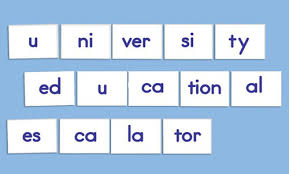
\includegraphics[scale=0.3]{syllabification.jpg}
  \end{flushright}
  
  \begin{flushleft}
  
\includegraphics[scale=0.5]{hts_logo.png}
  \end{flushleft}
  
  
\end{frame}
